\newcommand{\cnn}{konvolúciós neurális hálózat}

\chapter{Konvolúciós Neurális Hálózatok}
Ebben a fejezetben bemutatom a \cnn ok (CNN) felépítését, használatát és néhány nevezetes modellt. A \cnn okat a legtöbb esetben képfeldolgozás terén használják. A projekt során is képfeldolgozást kell megvalósítani, így ezek ismerete elengedhetetlen.

\section{Szerkezet}
Egy alapvető \cnn nak három alkotóeleme van. Először a képen a konvolúciós rétegek 2D konvolúciót végeznek. Ezt a műveletet többször is elvégzi a hálózatok, a következő konvolúció bemenete mindig az előző kimenete lesz. Néhány konvolúció után a pooling következik. Ez a két művelet ismétlődhet többször is akár. Ezek után a teljesen összekötött réteg következik, ami a kimenetet állítja elő. Az itt bemutatott általános \cnn osztályozó funkciót tud leghatékonyabban megvalósítani.

\begin{figure}[!ht]
    \centering
    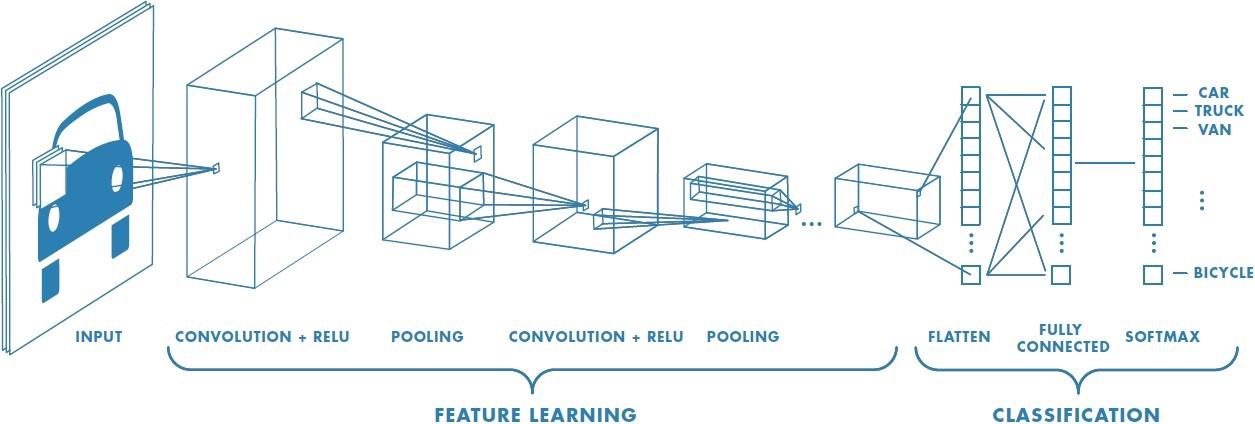
\includegraphics[width=150mm, keepaspectratio]{figures/cnn.jpeg}
    \caption{Egy konvolúciós neurális hálózat \cite{nnpic}}
\end{figure}

\subsection{Konvolúciós réteg}
Ebben a rétegben kétdimenziós konvolúciót végzünk a feldolgozandó képen. Ennek során először választunk egy kernelt. A kernel négyzetes mátrix, a képnél általában jóval kisebb mérettel. Gyakori kernelméret például a 3x3-as, vagy 5x5-ös mátrix. Alapvetően a kernel végighalad minden képkockán, és a középső pixelnek ad egy új értéket a kernel és a pixelek értékei alapján.

\begin{figure}[!ht]
    \centering
    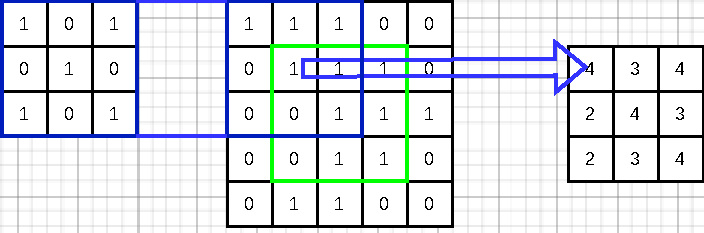
\includegraphics[width=150mm, keepaspectratio]{drawings/conv.drawio.pdf}
    \caption{2D konvolúció}
\end{figure}

Vegyük például a következő 3x3-as kernelt és egy kép 5x5-ös részletét. Az ábrán bal oldalt található a kernel, középen a bemeneti kép, jobb oldalon pedig a kimeneti kép. A képnek a zölddel jelölt részét tudjuk csak leképezni anélkül, hogy a kernel kimutatna a képen kívülre. Ezen a területen a kernel közepét a egy számmal helyettesítjük. Ezt a számot úgy képezzük, hogy a kernel értékeit megszorozzuk az fedésben lévő pixellel, majd ezeket az értékeket összeadjuk. Az új képen a kernel közepét ezzel az értékkel helyettesítjük. Ezután eggyel jobbra toljuk a kernelt, a sorvéget elérve pedig a következő sor elejére helyezzük.

Sok esetben szeretnénk csökkenteni a képek méretér a konvolúció során, hogy gyorsítsuk a hálózatot. Ehhez a konvolúció stride paraméterét kell növelnünk. A stride alapesetben 1, és azt jelzi, hogy a művelet elvégzése után mennyivel toljuk arrébb a kernelt. Könnyen belátható, hogy minél nagyobb a stride, annál kevesebb lesz a kimeneti pixelek száma, így csökken a kép mérete.

Jellemzően több konvolúció történik egymás után. Az első ilyen réteg feladata az alacsony szintű elemek megtalálása, például élek vagy színváltások megkeresése. Ahogy egyre több konvolúció történik egymás után, a hálózat egyre magasabb szintű jellegzetességeket fog tudni felismerni. Így már ebben a fázisban is az emberi megértéshez hasonlóan dolgozza fel a képeket a neurális hálózat.
\cite{ConvNetExplain}

\subsection{Pooling réteg}
A pooling rétegek feladata a bemenetük méretbeli csökkentése. Nagyon hasonlóan működnek a konvolúciós rétegekhez, a pooling rétegekben is egy kernel iterál végig a képen. Jellemzően egynél nagyobb stride értékkel.

A különbség a kernel értékeiben mutatkozik leginkább. Kétféle pooling-ot fordul elő gyakran. Átlag pooling esetében a kernelt az általa fedett pixelek átlagával helyettesítjük, maximum pooling esetében pedig a fedett pixelek közül a legnagyobbal. A maximum pooling a leggyakrabban használt a kettő variáció közül.

A pooling lényege tulajdonképpen a képen található domináns sajátosságok kinyerése. Ezekről a részekről forgatásra és pozícióra nézve invariáns információt tárol el a hálózat.\cite{ConvNetExplain}

\subsection{Teljesen összekötött réteg}
A teljesen összekötött réteg bármilyen neurális hálózat alapvető építőeleme. Ha a művelet kimenete nem egy másik kép, hanem valamilyen szöveges információ, például a képen látható objektum klasszifikációja, akkor a teljesen összekötött réteg végzi el az osztályba sorolás műveletét.

\begin{figure}[!ht]
    \centering
    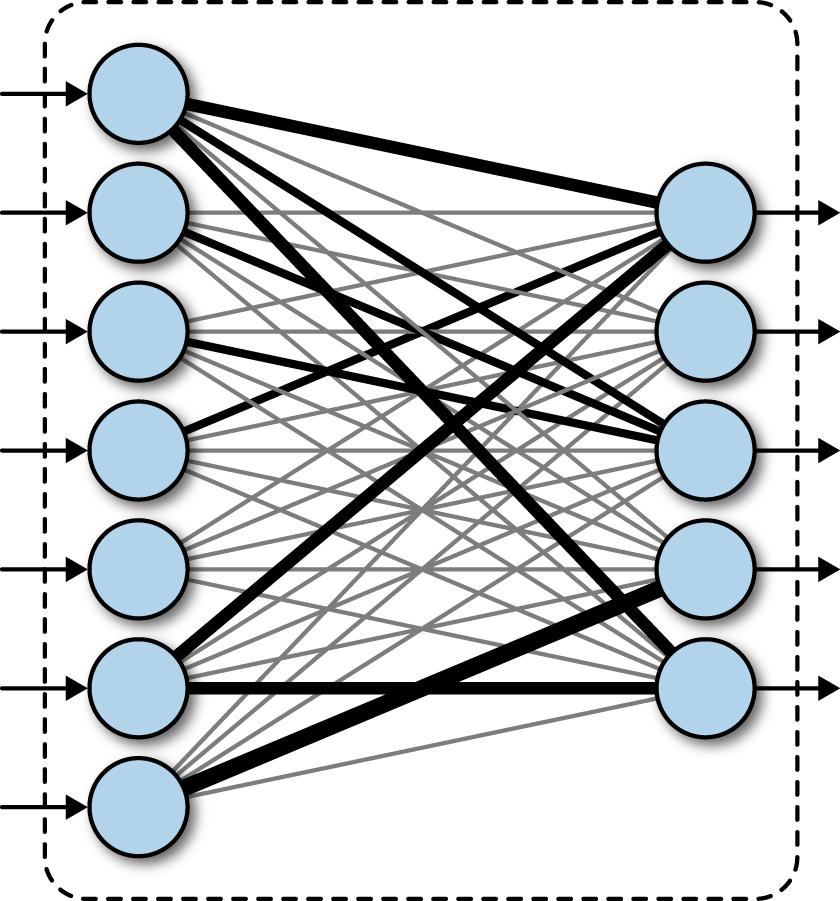
\includegraphics[width=80mm, keepaspectratio]{figures/fcl.png}
    \caption{Egy teljesen összekötött réteg \cite{ConvPic} }
\end{figure}

Ebben a rétegben két csoportba rendezve láthatunk neuronokat. A csoportok minden tagja össze van kötve a másik csoport összes tagjával és az összeköttetéseken súlyokat találunk. A képen a súlyokkal a vonalak vastagsága arányos. A jobb oldali csoport összes neuronja összegzi a bele futó élek végén található neuronok kimeneteit az éleken található értékekkel súlyozva, és az összeg lesz ennek a neuronnak a kimenete.

Ilyen rétegből is jellemzően több helyezkedik el egymás után. A legutolsó réteg a kimeneti réteg. Osztályozás esetén annyi kimeneti neuron van, ahány lehetséges osztály közül kell választani. Amelyik kimeneti neuronnak a legnagyobb az értéke, az ahhoz tartozó osztályba fogja sorolni a hálózat a bemeneti képet.

Felmerülhet kérdésként, hogy hogyan jutunk el egy képtől neuronokig. A kép a konvolúciós és pooling rétegekben folyamatosan egyre kisebb lesz méreteit tekintve. Egy ponton már olyan kicsi, hogy minden egyes pixelét tekinthetjük egy neuronnak, és felfoghatjuk a legelső teljesen összekötött réteg bemeneteként. A teljesen összekötött rétegek is jellemzően egymás után egyre kevesebb neuront tartalmaznak.

\section{Előre tanított neurális hálózat modellek}

A neurális hálózatok felhasználásának két lépése van. Először mintaadatok segítségével tanítani kell a hálózatot, ezután lehet csak kiértékelésre használni. A jelenlegi feladatnak csak a kiértékelés része az érdekes, ezt tudjuk ugyanis hatékonyan elvégezni a célhardveren.

Tanítás nélkül is van lehetőségünk neurális hálózatok felhasználására. Ebben az esetben ugyan nem tudjuk meghatározni, hogy milyen feladatot végez el a hálózat, azonban sok gyakori felhasználásra már rendelkezésre áll erősen optimalizált és teljesen tanított hálózat. Ezeket az előre tanított hálózatokat sok esetben van lehetőségünk áttanítani valamilyen másik, hasonló célra, azonban ebben a feladatban ilyen áttanítás nem lesz szükséges.

A Xilinx eszközök már sok esetben alkalmasak neurális hálózatok kiértékelésére. A cég mindenki számára elérhetővé tesz bizonyos neurális hálózat modelleket, amik olyan formátumban vannak, amiket Xilinx eszközön módosítás nélkül fel lehet használni kiértékelésre.
\cite{ModelZoo}

\subsection{Resnet50}
A modell teljes neve: \mycode{cf\_resnet50\_imagenet\_224\_224\_7.7G\_2.0}. A név a következő információkat tartalmazza: A modell caffe keretrendszerben volt tanítva az imagenet adathalmazon, resnet50 architektúrájú, és 224x224 pixel méretű képeken tud dolgozni. Ez a hálózat a bemenetére adott képet osztályozni tudja 10 lehetséges csoport közül egybe.

A feladatom első részében ezt a modellt használtam a rendszer tesztelésére, a pontos folyamatot a későbbiekben fogom bemutatni.

\subsection{Facerec}
A feladat további részeiben arcfelismerést és bounding box rajzolást kell majd elvégezni. A Model Zoo-t végignézve több lehetőség is adódik, ezek közül részletesebb tesztelés után fogok konkrét modellt választani. Mindegyikre igaz azonban, hogy a facerec arcfelismerő architektúrát valósítják meg. A különbség a bemeneti kép méretében, a tanító keretrendszerben és a tanításra felhasznált adathalmazban van.


